\documentclass{sigchi}

% Use this section to set the ACM copyright statement (e.g. for
% preprints).  Consult the conference website for the camera-ready
% copyright statement.

% Copyright
%\CopyrightYear{2018}
%\setcopyright{acmcopyright}
%\setcopyright{acmlicensed}
%\setcopyright{rightsretained}
%\setcopyright{usgov}
%\setcopyright{usgovmixed}
%\setcopyright{cagov}
%\setcopyright{cagovmixed}
% DOI
%\doi{http://dx.doi.org/10.475/123_4}
% ISBN
%\isbn{123-4567-24-567/08/06}
%Conference
%\conferenceinfo{CHI'16,}{May 07--12, 2016, San Jose, CA, USA}
%Price
%\acmPrice{\$15.00}

% Use this command to override the default ACM copyright statement
% (e.g. for preprints).  Consult the conference website for the
% camera-ready copyright statement.

%% HOW TO OVERRIDE THE DEFAULT COPYRIGHT STRIP --
%% Please note you need to make sure the copy for your specific
%% license is used here!
% \toappear{
% Permission to make digital or hard copies of all or part of this work
% for personal or classroom use is granted without fee provided that
% copies are not made or distributed for profit or commercial advantage
% and that copies bear this notice and the full citation on the first
% page. Copyrights for components of this work owned by others than ACM
% must be honored. Abstracting with credit is permitted. To copy
% otherwise, or republish, to post on servers or to redistribute to
% lists, requires prior specific permission and/or a fee. Request
% permissions from \href{mailto:Permissions@acm.org}{Permissions@acm.org}. \\
% \emph{CHI '16},  May 07--12, 2016, San Jose, CA, USA \\
% ACM xxx-x-xxxx-xxxx-x/xx/xx\ldots \$15.00 \\
% DOI: \url{http://dx.doi.org/xx.xxxx/xxxxxxx.xxxxxxx}
% }

% Arabic page numbers for submission.  Remove this line to eliminate
% page numbers for the camera ready copy
% \pagenumbering{arabic}

% Load basic packages
\usepackage{balance}       % to better equalize the last page
\usepackage{graphics}      % for EPS, load graphicx instead 
\usepackage[T1]{fontenc}   % for umlauts and other diaeresis
\usepackage{txfonts}
\usepackage{mathptmx}
\usepackage[pdflang={en-US},pdftex]{hyperref}
\usepackage{color}
\usepackage{booktabs}
\usepackage{textcomp}

% Some optional stuff you might like/need.
\usepackage{microtype}        % Improved Tracking and Kerning
% \usepackage[all]{hypcap}    % Fixes bug in hyperref caption linking
\usepackage{ccicons}          % Cite your images correctly!
% \usepackage[utf8]{inputenc} % for a UTF8 editor only

% If you want to use todo notes, marginpars etc. during creation of
% your draft document, you have to enable the "chi_draft" option for
% the document class. To do this, change the very first line to:
% "\documentclass[chi_draft]{sigchi}". You can then place todo notes
% by using the "\todo{...}"  command. Make sure to disable the draft
% option again before submitting your final document.
\usepackage{todonotes}

% Paper metadata (use plain text, for PDF inclusion and later
% re-using, if desired).  Use \emtpyauthor when submitting for review
% so you remain anonymous.
\def\plaintitle{OutTest}
\def\plainauthor{Armando João da Silva Gomes}
\def\emptyauthor{}
\def\plainkeywords{OutSystems; software testing; automated testing; automated test generation; low-code.}
\def\plaingeneralterms{Documentation, Standardization}

% llt: Define a global style for URLs, rather that the default one
\makeatletter
\def\url@leostyle{%
  \@ifundefined{selectfont}{
    \def\UrlFont{\sf}
  }{
    \def\UrlFont{\small\bf\ttfamily}
  }}
\makeatother
\urlstyle{leo}

% To make various LaTeX processors do the right thing with page size.
\def\pprw{8.5in}
\def\pprh{11in}
\special{papersize=\pprw,\pprh}
\setlength{\paperwidth}{\pprw}
\setlength{\paperheight}{\pprh}
\setlength{\pdfpagewidth}{\pprw}
\setlength{\pdfpageheight}{\pprh}

% Make sure hyperref comes last of your loaded packages, to give it a
% fighting chance of not being over-written, since its job is to
% redefine many LaTeX commands.
\definecolor{linkColor}{RGB}{6,125,233}
\hypersetup{%
  pdftitle={\plaintitle},
% Use \plainauthor for final version.
  pdfauthor={\plainauthor},
%  pdfauthor={\emptyauthor},
  pdfkeywords={\plainkeywords},
  pdfdisplaydoctitle=true, % For Accessibility
  bookmarksnumbered,
  pdfstartview={FitH},
  colorlinks,
  citecolor=black,
  filecolor=black,
  linkcolor=black,
  urlcolor=linkColor,
  breaklinks=true,
  hypertexnames=false
}

% create a shortcut to typeset table headings
% \newcommand\tabhead[1]{\small\textbf{#1}}
% End of preamble. Here it comes the document.
\setcopyright{none}
\begin{document}

\title{\plaintitle}

\numberofauthors{1}
\author{%
  \alignauthor{Armando João da Silva Gomes\\
    \affaddr{Instituto Superior Técnico}\\
    \affaddr{Lisboa, Portugal}\\
    \email{armando.gomes@tecnico.ulisboa.pt}}\\
}

\maketitle

\begin{abstract}
The rapid growth of the IT market needs and the increasing complexity of software projects led to a talent shortage. Companies in need of resources tend to hire either junior developers or people with no background in software development as well as choosing low-code platforms for development. The lack of skills - although softened due to the features of low-code platforms - lead to defective development, defective quality assurance process and, in the end, a defective software system. One of the methods to improve the quality assurance process is through automated software testing. The current offerings for the OutSystems platform lack the required functionality and/or require additional developments that represent a significant overhead to project planning in terms of schedule and budget. In this work, a framework for automated test case generation in the OutSystems platform is proposed. This framework targets the Core Business layer in OutSystems proposed 4-Layer Canvas.
\end{abstract}

\category{D.2.5}{Software Engineering}{Testing and Debugging}

\keywords{\plainkeywords}

\section{Introduction}

Building software is an expensive and demanding task. When companies cannot find exactly what they are looking for - usually, a commercial off-the-shelf solution -, they have no alternative than to build it from scratch. Whether companies tend to build it themselves or hire another company to do so (outsourcing), is a decision that might depend on the organizational maturity, application domain and in-house knowledge, flexibility, time constraints, value and overall productivity\cite{buildbuyoutsource}. Additionally, when building in-house software, companies tend to fall into the \textit{sunk cost effect}, in which decision-makers are heavily influenced by the investment already made\cite{effectsofsunk:keil}. In order to reduce costs and increase the productivity, companies tend to embrace low-code platforms and their bold promises of delivering software multiple times faster. This introductory chapter will identify some of the factors that influence the software cost and quality and how low-code platforms give response to current software development needs.

So, why is the software development process so expensive? There are various reasons for that. The single biggest reason is the development team. According to Glassdoor, the average software engineer in Portugal costs around 25.000 to 30.000 EUR per year. If a company needs 10 people to develop a single project, just the development team costs can go over 250.000 or even 300.000 EUR, depending on the member profiles. Other factors include the complexity, the required time-to-market, the required expertise and so on. Finally, one additional factor that influence the cost is the failure rate. 
The Standish Group produces an yearly report with the state of the IT projects, with the first report published in 1994\cite{CHAOS1994}. This report already had very interesting mentions regarding IT application development: in the United States, the average number of projects per year was 175.000, leading to a total cost of over 250 billion USD. The impressive information comes next: of those 175.000 projects, around 31.1\% of them were canceled before being concluded and 52.7\% ended up costing more than 189\% of their original estimates. In terms of successes, only 16.2\% of the projects were being completed on-time and on-budget. The costs associated with building custom software don't end once the software is built - applications usually require constant evolution and maintenance, which also helps in increasing overall costs.
But which factors influence the software cost?

Two of those factors are software complexity and the current skill shortage. Determining the complexity in a software system may be considered a subjective term. A study by McNicholl and Magel in 1982\cite{McNicholl:1982:SNP:800049.801785} has shown that the perception of the complexity of software varies from individual to individual, that it may be influenced by the size of the result than the expended effort and, finally, that doesn't seem to be any measurable individual characteristic that could allow the prediction of  previous statements.
In an article by Robert Glass titled "Sorting out software complexity"\cite{Glass:2002:SOS:581571.581584}, the author has conducted a research and has reached two interesting findings: \textit{for each 25\% increase in the problem complexity, there is a 100\% increase in the complexity of the software solution} and that \textit{explicit requirements explode by a factor of 50 or more into implicit (design) requirements as a software solution proceeds}.

\subsection{Low-code platforms}
The low-code market is on the rise and its worth is estimated to grow from 3.2 billion USD in 2016 to approximately 27.23 billion USD in 2022, a compound annual growth rate of almost 45\%. In terms of valuation, the latest round of funding for OutSystems has introduced the company into the "unicorn list" - a list containing companies valued at more than one billion USD.

The term low-code is a new term for a concept that has been around for long. The notion of "power user" or "citizen developer", people who can optimize their workflow by themselves,  inside companies is wildly known, with these platforms aiming at reducing the entry barrier for the average employee\cite{12436424020170801}. Usually, platforms that focus only on the average employee are called no-code platforms, in which no coding is required and the all the available features are already present in it. On the other hand, the pure low-code platforms target traditional developers and IT people.
A low-code platform allows a developer to build an application - usually web and/or mobile - faster due to the nature of the already available components. Additionally, if any specific requirement is needed, these platforms allow the developer to extend the platform with the given functionality - hence the difference between low-code and no-code. 

\subsection{Popularity of low-code platforms}
According to Forrester, a research and advisory firm, there are three key factors that highlight the real value of these platforms\cite{forresterwavelowcodeq4}:
\begin{itemize}
	\item \textbf{Speed up application and innovation delivery} Based on Forrester July 2017 survey, 31 of 41 Application Development and Delivery (AD\&D) leaders stated that traditional coding meant huge difficulties to meet business requirements on time while 21 of 41 also stated that the lack of flexibility was a challenge and, finally, 20 of 41 AD\&D leaders stated that traditional coding means a long time to update existing applications. Related to the delivery speed on the low-code platforms, 40 out of 41 AD\&D leaders stated that they have seen a notable or significant improvement while only one (1) AD\&D leader stated that only a marginal improvement was seen. This data shows that low-code platforms allow teams to dramatically raise their productivity and ability to response in time to demands for business software.
	\item \textbf{Prove useful for large-scale applications} One common misconception about the low-code platforms is that are only good for \textit{departmental} (code for small, non-critical) applications. Many of the adopters of these platforms have built and use these applications corporate-wide or in multiple departments.
	\item \textbf{Contribute to Application Development and Delivery move to public clouds} According to recent studies\cite{forresterpubliccloudmarket}, the adoption of public cloud services - either from full applications (i.e. Atlassian's JIRA) to infrastructure services (i.e. Amazon Web Services) - has been and is expected to keep growing, hitting a 23.6 billion USD valuation in 2020. Since these low-code platforms have publicly accessible clouds for development and delivery, they have emerged as a one of three major Platform-as-a-Service options.
\end{itemize}
Still related to speeding up the application delivery, low-code automation allows users to create and deploy high-quality web and mobile applications significantly faster – typically in weeks rather than months. According to OutSystems, gains in productivity can achieve up to 600\% - or six times faster.

Enabling IT departments to meet the growing demand for the rollout of new applications is only one of the benefits of low-code platforms since these platforms also streamline application maintenance and updates. This is critical, given today’s rapidly changing business needs. If the low-code platform is robust, it can also integrate readily with existing IT infrastructure meaning that migration and legacy enterprise systems are much less of a concern. In addition, users of these platforms can manage integration for easy access and replication, resulting in ongoing efficiency. An article written by Jon Idle\cite{benefitsoflowcode} explains the rational of when and why use low-code platforms. According to the article, low-code platforms need to be considered when there's the need to build or manage multiple applications for a business in a quick manner, with proper life cycle management and/or for multiple platforms. Besides the tangible results of developing in these platforms, there is also a greater stakeholder engagement and satisfaction - since they can iterate and see progress more frequently -, a lower risk and higher return on investment as well as, to certain extent, an elimination of the IT skills gap.

\subsection{Motivation}
According to the World Quality Report 2017-18\cite{wqr1718}, in 2017 companies allocated 26\% of their total IT budget to quality assurance (QA) processes. This value, despite being considerable, means a five percent decrease (31\%) from 2016 and a nine percent decrease (35\%) from 2015. In terms of the overall cost, building software has an immediate and a future cost. While the former depends mainly on the duration, scope and resources, the latter depends not only on the same but it also depends on the effectiveness of the QA process.
The cost of software testing has a visible face: people will often take the biggest share of the budget but sometimes there's the need to license the bug tracking platform - like JIRA, for instance - or even some tools for testing - for instance, UI testing, load testing and others.
But what about the "hidden costs" of the software testing? An article published in 2002\cite{718084420020805} concluded that bugs or errors had an annual cost of 59.5 billion USD. Another interesting fact is that almost 38\% of that cost (22.5 billion USD) could be likely removed if the testing infrastructures would be improved. These costs represent if the errors would be found near to development stages - the sooner, the better - but, unfortunately, most of the errors were found late in the process.
Related to when is an error found and the relative cost, Steve McConnel has detailed the subject in his book \textit{Code Complete}\cite{McConnell:2004:CCS:1096143}. It is stated that an issue introduced in the requirements and design phase could cost from 1 to 100 orders of magnitude while an error introduced in the development phase can cost from 1 to 25 orders of magnitude. It is safe to conclude that QA process plays a vital role in terms of a project or a company's budget since it can save much more than it costs.

\subsection{Problem}
Due to the nature of low-code platforms, project managers look into their usage so they can reduce costs in two different vectors: development time is cut and, due to a lower learning curve, less skilled developers can be hired. Although it is expected that applications built with low-code platforms contain less bugs, they are not bug-free and, as a result, it is required to have a proper QA process in place. Despite providing huge benefits in terms of application development \textit{per se}, they lack "low-code" testing capabilities: developers still need to manually implement their own unit tests. How can be assured that, due to the lack of proper QA skills of developers, the designed test suite is appropriate and the software is released with the desired quality? 
\subsection{Objectives}
Considering the current talent shortage along with developers without the required skill set in order to assure the effectiveness of the QA process, the objective of this work is to produce a framework able to automatically generate and execute test suites for a given application built with the OutSystems platform. The main requirements for this framework are:
\begin{itemize}
    \item Allow the developer to import and select the module under test.
    \item Generate full test suites for all the methods/actions present in a given module.
    \item Allow the developer to run the mentioned test suites, either on demand or in a given schedule.
    \item Provide execution reports for scheduled tests.
\end{itemize}
Additionally, it is important that this framework has a set of additional requirements in terms of performance, usability and size. These requirements are:
\begin{itemize}
    \item The framework should provide an User Interface that is easy to use and that allows an easy understanding of the current state of the system, following Nielsen's Heuristics\cite{Nielsen:1994:EEP:191666.191729}.
    \item The framework should provide reasonable performance in terms of test execution, meaning that the productivity flow of a developer should not be affected by a given test execution - either on demand or
    scheduled.
    \item The framework should provide real-time results for a given test case/suite execution.
    \item The framework should be as small as possible in terms of OutSystems licensing, aiming for a reasonable 50 Application Objects in size\footnote{Application Objects are elements of the application and are used as a measure for licensing purposes.}.
\end{itemize}
\subsubsection{Why OutSystems?}
There are several reasons for choosing the OutSystems platform, with the most relevant being the daily development tool of the author. Additionally, the OutSystems platform is a world-renowned portuguese company that, in October 2018, has over 245 partners and more than 167.000 community members, being present in 52 countries and 22 different industries. In the low-code platform ecosystem, OutSystems is a founder and also considered a leader with a strong platform and big ambitions. The platform has received multiple awards, including the top rated low-code platform by TrustRadius and four times the CODiE award by SIIA: three for the best mobile application development platform and one for best could platform as a service. There are some features that highlight the advantages that the OutSystems Platform provides and make it a serious contender when a low-code or no-code platform is considered: rapid productivity, multi-channel development, reduced costs and no lock-in approach.

\textbf{Despite several attempts, the work presented was not supported by OutSystems, limiting the end result to some extent. There were, however, some resources provided in order to streamline some of the progress.}

\section{OutSystems Platform}
The OutSystems platform is a low-code solution for the complete application development life cycle. OutSystems achieves this by allowing developers and teams to respond to critical business requests for demanding market needs. A development team can design, develop, assure quality and analyze and manage an application, independently of the size of it. As such, the platform provides a front to end development solution while also allowing deployment and maintenance needs. In the end, the goal of the OutSystems platform is to provide reduced risks and costs associated to software development by implementing a continuous delivery approach.

\subsection{Product overview}	
\begin{figure}[h!]
	\centering
	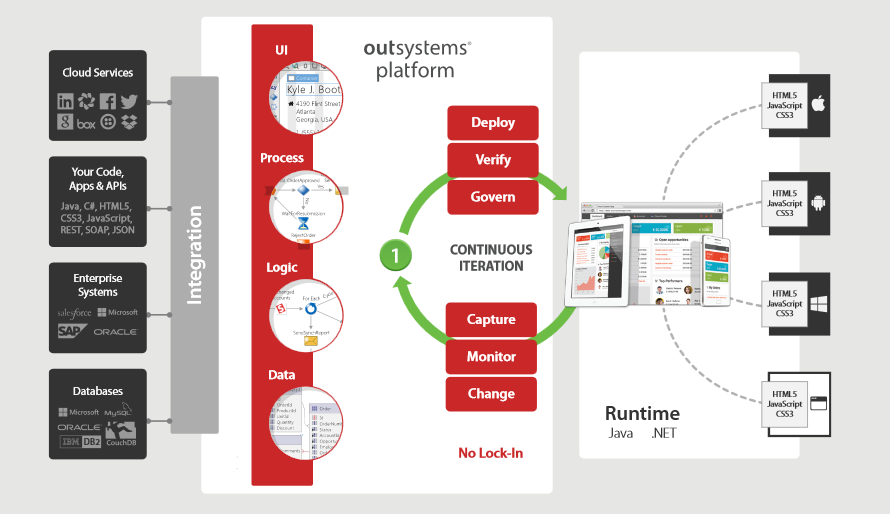
\includegraphics[width=0.9\columnwidth]{outsystems-architecture}
	\caption{OutSystems platform high-level architecture}
\end{figure}
		
Internally, the OutSystems platform provides environments, tools and components that streamline software development, covering all life cycle steps. In terms of the environments, the two most important are:

\begin{itemize}
    \item \textbf{Visual development environment - Service Studio} Service Studio is the IDE used to create all parts of the application stack: database structure, application logic, user interfaces, business processes, external integrations and security policies.
    \item \textbf{Integration environment - Integration Studio} Integration Studio is an environment used for component creation that extend the platform, i.e., external databases, specific snippets of code and third-party systems.
\end{itemize}		
 
The developments done within these two environments will reside in a third environment, the platform server. The OutSystems platform Server is the server component and the core of the platform. This server does the process of generation and optimization of code as well as the compilation and deployment of it. Besides this, it is also responsible for batch jobs as well as application logs.

\begin{figure}[h!]
    \centering
	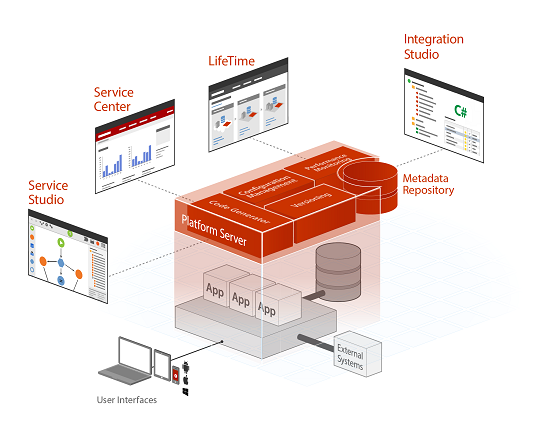
\includegraphics[width=0.9\columnwidth]{platform-server}
    \caption {The various components of the platform server in the overall OutSystems platform architecture}
    \label{fig:platformserver}
\end{figure}

When the development is finished and the application is ready for the next step of the life cycle, there are two additional resources that aid in the team: \textbf{Service Center}, which is a management console for the operational aspects of the environment - i.e. connection strings, web service endpoints - and \textbf{LifeTime}, which is a console for centralized management for development, quality assurance and production environments.

In terms of the development task, the visual development environment (Service Studio) allows developers to drag and drop elements to create the UI as well as business logic and data structures. Adding to this ease of use, Service Studio has a full reference-checking and self-healing engine that prevents errors in the applications when changes are made.  Although there is a reasonable set of available elements that developers can use, if these elements are not sufficient to achieve the desired result, they can go on and extend the platform with their own code.

The continuous delivery approach is, in simple terms, achieved by the click of a button: 1-click publish. When this functionality is used, the development environment allows the developer to manually or automatically merge his changes into the published version, replacing the current code and making it available right away. When the merge is complete - if necessary -, various services are invoked:

\begin{itemize}
    \item \textbf{Code Generator} The code generator service converts the OutSystems modeling language modeled in the development environment and generates the native .NET (or Java) code. The reason for this is that generated applications are optimized for performance and security by executing on top of standard environments.
    \item \textbf{Deployment Service} Once the code generator finishes its job, the deployment services deploy the generated code into a standard web application server. This standard server is, usually, either Microsoft Internet Information Services or RedHat's JBoss. This service, during the deployment procedure, ensures that the application is consistently installed across all servers.
    \item \textbf{Application Services} During the whole process of generating, deploying and executing the application, the application services provide and manage the execution of batch jobs and logging features for the platform/applications. These logging features could go from simple audit messages to errors or performance indicators.
\end{itemize}
Along with this process of generating and compiling the application, an application model is created and is stored in the same platform server, using a built-in version control system and a dependency analysis is made. In the event that another application might be affected by the changes being applied, the system notifies the team accordingly.

\subsection{Architectural principles}
OutSystems uses a pattern called 4-Layer Canvas (4LC) which helps the architect to design a Service-Oriented Architecture in a simple manner to attain simple goals: it suggests - and encourages - the abstraction of services and the correct isolation of distinct functional modules in order to promote module reusing.

\subsubsection{The layers}
As the name of the architecture pattern suggests, there are four different layers, each with its own purpose. From bottom to top:
\begin{itemize}
    \item The \textbf{Library Layer} contains business-agnostic services to extend the framework/functionality with highly reusable assets, UI Patterns, connectors to external platforms and systems and, additionally, integration of native code (C\# in case of the web component, Objective-C/Swift and Java for the mobile part).
    \item The \textbf{Core Layer} aims to provide the isolation of business modules, exposing reusable entities, business rules and business widgets.
    \item The \textbf{End User Layer} provides user interfaces and processes (BPM processes or, in OutSystems terminology, Business Process Technology processes), reusing the modules from the Library and Core layers in order to implement the user stories.
    \item Finally, the \textbf{Orchestration Layer} contains processes, dashboard and home pages in order to provide a unique and unified user experience.
\end{itemize}

\subsection{Core Layer}
The Core Layer, Core Business Layer or even Core Services layer is the most important layer in an OutSystems application architecture. The decisions made during the design and, most important, the coding that is done during the development phase, hugely influence not only the outcome of the project but other factors like scalability, reusability and performance. 

A typical module in this layer will be composed of entities - which is an element that allows information to be persisted in the database - and server actions, which can do CRUD operations  or any other business logic, like calculating a currency exchange rate or a loan interest rate.

This Core Layer is the central part of this work. The testing framework that was produced aims to allow the unit testing of these server actions without requiring any further developments. As of now, in order to test these actions it needs to happen one of two things: "wait" until the user interface is implemented so the logic can be tested - typifying as integration testing instead of unit testing - or implement a test case using regular development practices.

\subsection{Domain-Specific Languages (DSL)}
Martin Fowler defines a DSL as "\textit{a computer programming language of limited expressiveness focused on a particular domain}"\cite{Fowler:2010:DSL:1809745}. Moreover, he identifies four key elements to this definition:
\begin{itemize}
    \item \textbf{Computer programming language} A DSL is used by humans to define instructions, therefore being a language easily understandable for humans but executable by a computer.
    \item \textbf{Language nature} A DSL should have a sense of fluency where the meaning comes not only from the individual elements but also from the way they are connected.
    \item \textbf{Limited expressiveness} A DSL should support only the minimum required of features to support its domain.
    \item \textbf{Domain focus} A DSL should be focused on a small domain, potentiating its worthfulness - this being as a consequence of the limited expressiveness.
\end{itemize}

Beyond the definition, he also defines three main categories in which DSL may fit: external DSL, internal DSL and language workbench.

The \textbf{external DSL} is defined as a separate language from the main language of the application it works with. It has its own language and it's parsed by a code on the host application. The \textbf{internal DSL} is a particular way of using a general-purpose language, in which only a subset of the language's features are used and, finally, a \textbf{language workbench} is an Integrated Development Environment for defining and building DSLs.

The OutSystems Modeling Language is an \textbf{external DSL} since it uses a separate language from the application it works with (HTML/C\# for the generated code) and uses a parser\footnote{The inner working of this parser is unknown since it's intellectual property of OutSystems and was not disclosed.} that generates the final code. This parser is also able to generate XML files - which are used in this work.

\section{Related Work}
As of October 2018, there is no solution that allows the automated test suite generation for User Actions in the OutSystems platform. There are, however, other existing solutions aimed at providing testing capabilities in the platform. But how to test actions in the OutSystems platform?

\subsection{Method scope testing}
The method scope testing is a deeper level of the class scope testing since here the parts that interoperate are statements. In other words, a method scope testing focuses on testing the relationship among statements. When testing classes, the common procedure is to send messages to one method at a time. Due to the nature of the OutSystems platform, user actions could be also called methods - thus being this mapping the bridge between object-oriented testing and OutSystems testing. A module, on the other hand, could also be considered as a class, although the similarities could not be so straightforward.
Binder states that although only one method at a time is tested, methods cannot exist apart from a class. Again, due the nature of the OutSystems platform, this is not entirely applicable. There is no need to have an implicit cooperation between methods, "living" each one on their own. This doesn't mean, though, that user actions cannot rely on other user actions - which is very common, indeed.
\subsubsection{Control Flow Graph and Coverage}
The Control Flow Graph is a representation of predicates - single or multiple conditions which evaluate to true or false - using graph notation. Each of the nodes represent a block of instructions while the edges represent a predicate. Computing predicates allow the developer to identify which values trigger the given branches and, thus, allowing to achieve acceptable levels coverage.
\begin{figure}[h!]
    \centering
	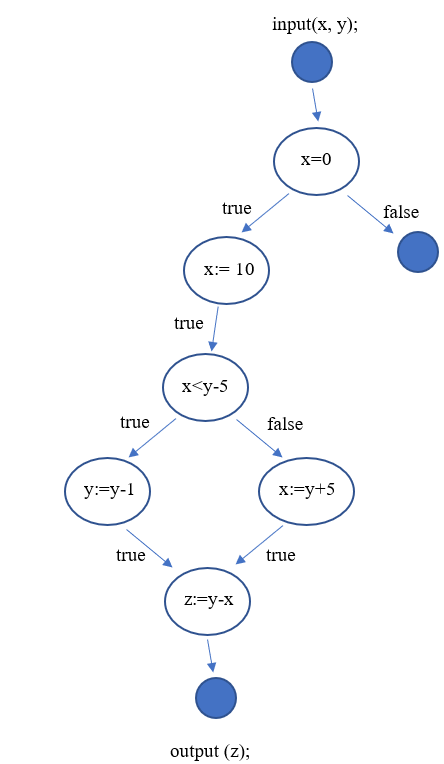
\includegraphics[width=0.9\columnwidth]{cfg}
    \caption {Control flow graph representation}
    \label{fig:cfg}
\end{figure}
Coverage models include \textbf{Statement Coverage}, \textbf{Branch Coverage}, Multiple-condition Coverage Object Coded Coverage, Basis-Path Coverage and Data Flow Coverage. For the scope of this work, it is important to understand Statement and Branch coverage models.

The statement coverage model, or C1, is calculated based on the number of statements of a given method that have been executed at least once. The branch coverage model, or C2, uses the number of branches that are executed, even if some statements in those branches are not executed.
According to Binder, in large systems achievable coverage lies between 80 and 85\%, with the remaining 15 to 20\% being due to unreachable code.

\subsection{Method scope test design patterns}
There are several patterns to design method scope tests although only the two most relevant will be presented. Each one applies to a specific purpose implemented by the method under test (MUT).
\subsubsection{Category-Partition}
The category-partition test pattern might be used on any given method or function in any given scope, being appropriate for any method that implements one or more independent functions. The intent of this pattern is to design a test suite based on input/output analysis.
This pattern assumes that faults are related to value combination of message parameters and instance variables. If faults are only visible through certain sequences, these pattern might not reveal them.

The strategy involves identifying all functions of the MUT followed by the identification of input and output parameters for each function, along with categories. Then, partition each category into choices considering existing constraints on said choices. Finally, the test cases are generated by enumerating all the possible combinations and the expected results are developed using an appropriate oracle.
Although being a fairly straightforward technique, the identification of categories and choices is a subjective process and the size of the generated test suite may become quite large.

\subsubsection{Combinational Function Test}
The combinational function test pattern is more appropriate for methods that implement complex algorithms, business rules or other case-based logic or, in other words, it aims to design test suites for behaviors based on state or message parameters.

The fault model of this pattern could be when incorrect values are assigned to decision variables, incorrect or missing operators/variables in predicates, incorrect structure in a predicate, incorrect or missing default case or default action and many others.

The strategy for this pattern is to create a decision table that lists which different input combinations will result in different actions, along with the expected response of the MUT. Each of the entries in the input combinations should only be boolean-type expressions and each combination of input variables and respective action is called a variant. In the case that decision variables are not boolean, additional tests should be made to exercise the boundaries.

This pattern highlights incorrect response actions to test messages and often reveals design errors and omissions. Additionally, faults resulting from the order of message to external dependencies or corruption of object variables hidden by the MUT interface may not be shown.

\subsection{Mocking}
When the MUT has any external dependencies, it is useful to use mocking so the developer can only focus on the code being tested and don't get concerned about the behavior of said dependencies. Mocking works by replacing dependencies with closely controlled objects that simulate the expected behavior. There are three types - or levels - of mocking:
\begin{itemize}
    \item \textbf{Fakes} allow the developer to replace the actual code of the external dependency by implementing the same interface but without further interaction with other objects. The results from said implementation are hardcoded and the need for new fakes increase as the test suite increase. Big test suites mean a fake structure that is hard to understand and maintain.
    \item \textbf{Stubs} is an evolution from fakes. While using fakes require implementing actual code for the external dependency, using stubs with a mocking framework allow the developer to create a stub with minimal amount of effort.
    \item \textbf{Mocks} is the most evolved mocking type. It is very similar to stubs - providing the same advantages - but allow the developer to set expectations on a given method - developer can define the output value for each method call, for instance. While stubs are "blind" substitutes, mocks allow the developer to verify its usage.
\end{itemize}

In order to use these types of mocking, a developer uses a mocking framework. Mocking frameworks are not substitutes of unit testing frameworks but rather complement them by isolating dependencies.
In terms of offerings, there are several free and commercial mocking frameworks. In terms of the free offering, JustMock Lite, NSubstitute, Moq and Rhino Mocks are the most publicized. Microsoft Fakes, included in Visual Studio is also a good option. In terms of commercial solutions, JustMock and Typemock seem to be the most complete offerings.

\subsection{Symbolic Execution}
The symbolic execution testing method is a technique where a program is analyzed to determine which set of inputs trigger a given part of a program\cite{King:1976:SEP:360248.360252}. It is not a recent technique, with articles proposing it in 1975\cite{Boyer:1975:SFS:390016.808445} but has always faced dificulties related to constraint satisfiability. The computed paths are created using an interpreter that, by using symbolic values instead of actual values, obtains a set of expressions for the program input variables that will \textit{hit} possible outcomes of conditional branches. There are some known limitations to this technique, though. For large programs, it might not be possible to execute all feasible paths\cite{Anand2008} and, while \textit{interpreting} a given application, it might not be possible to control environment interactions, causing consistency problems - KLEE\cite{Cadar:2008:KUA:1855741.1855756} and Otter\cite{otter} are some tools used to mitigate issues related to environment interactions.
Other challenges are memory handle, path explosion and constraint solving\cite{SurveySymExec-CSUR18}.

\subsubsection{Constraint Solving}
In order to understand exactly which values of input data are required so a given branch can be execised, it is often used a constraint solver on the computed paths. A constraint solver is a decision procedure for logical formulas expressing problems. Two common solvers are the boolean satisfiability problem (SAT) and the Satisfiability Modulo Theory (SMT) solvers. The SMT solver is an extension to the SAT in which instead of being based on boolean logic, it evolved into first-order logic\cite{6713475020110901}.
An approach for automatically generate test data using constraing solving techniques was proposed by Gotlieb, et al.\cite{Gotlieb:1998:ATD:271775.271790} One example of a solver implemented for the .NET platform is the Z3 Theorem Prover.

\subsection{Solutions for the OutSystems platform}
As stated previously, there are no solutions for the OutSystems platform for which no further developments are required in order to test user actions.

\subsubsection{Unit Testing Framework}
The Unit Testing Framework is a framework for unit test definition created by Andrew Burgess and published, for the first time, in June 3rd, 2013. The last update was published by Paulo Ramos in April 5th, 2016 and it has not been updated for the last installments of the Platform (v10 and v11).
This framework provides a set of functions that the developer can use when designing the tests. As suggested, this framework does not provide automated test case generation since it targets a "design-time" level instead of a "run-time" level. This can mimick what is done using a Test Driven Development\cite{Astels:2003:TDD:864016} approach in other programming languages like Java or \texttt{C\#}. The main difference is that it requires the signature of the function to be created beforehand, in order to be imported into the test case.
The set of functions offered by this framework is a standard one, offering functions for the typical \textit{assert equals} and \textit{assert fail/pass} as well as others like \textit{assert is true/false}, \textit{assert pass} and, finally, \textit{assert contains text}.

\subsubsection{BDD Framework}
The BDD Framework is a testing framework that provides a set of tools for easily creating Behavior Driven Development tests for an OutSystems application. The Behavior Driven Development is the base concept of the application, following the principles of the \textit{Given}, \textit{When} and \textit{Then}. This framework allows the user to define the scenarios and then each step of the scenario. These steps require a specific development for each one, an activity that can be time consuming and might require additional development depending on the pre or post-conditions that are required.
As such, depending on the type of the tests that the developer wants to do, designing and implementing the test might require additional developments to assure required data is present and the test can proceed.
Similarly to the Unit Testing Framework, the BDD Framework also provides common assert functions, namely: \textit{assert}, \textit{assert fail}, \textit{assert true/false}, \textit{assert value}. Unfortunately, it has some limitations that difficult it's adoption: designing the tests can consume a lot of Application Objects; it doesn't support scheduling of tests and it doesn't provide an overall report based on test execution. It also doesn't support automated test generation.
An analysis on the recent information and blog posts by OutSystems on the software testing subject leads to conclude that testing using Behavior Driven Development is the suggested way for OutSystems applications.

\subsubsection{Test Framework}
The Test Framework is an open source application that offers simple management and automated execution of OutSystems Unit and API tests. With seamless integration with BDD Framework and Unit Testing Framework, it allows automated regression tests setup and execution. This component has been developed by Indigo and supports the following set of features:
\begin{itemize}
	\item \textbf{Manage Test Suites, Cases and Steps} Define test scenarios, for both Unit and API tests, and it executes them manually or daily at a given schedule.
	\item \textbf{Test execution classification} Classify test executions as Broken or Defect, to help teams focus on fixing tests, or actually fixing the wrong functionality identified by the test.
	\item \textbf{Introspection and execution of BDD and UTF Tests} Automatically imports and runs BDD or Unit Test Framework tests periodically, validating results on every run.
	\item \textbf{Quality overview} Monitor the evolution of defined test suites, gaining a clear understanding of whether tests are not designed for maintainability, or if the applications are increasingly having more quality and less regressions.
\end{itemize}
The documentation for this Test Framework is provided by OutSystems and it doesn't seem to have huge adoption - only 131 downloads since the release, in September 27, 2017. Also, the Application Object consumption is of 83 AO's, which is a significant amount for the OutSystems Platform - although AO's are usually unlimited in development environments.
On a usage-basis, this tool requires BDD Framework to manage and execute the tests, seeming like an extension to the said framework. This tool, like the others, doesn't support automated test generation.

\subsubsection{Automator}
The Test Automator is a browser (based on Selenium) and unit (based on web services) regression testing tool for the OutSystems Platform. It was built for OutSystems Platform version 7. The last update for this component was released in November 16th, 2015 by Paulo Garrudo and, in total, it counts 686 downloads since its initial release.
This tool allows the usage of Selenium test scripts as well as some OutSystems logic though it's most focused for UI testing instead of logical testing. This logical testing capabilities are well limited - it requires to be exposed on a web service and it has to follow a certain structure. Eligible logic methods should have no input parameters and should return only one output parameter, parameter that needs to be a single boolean or text.

\section{Solution}
Due to the nature of the OutSystems Modeling Language (OML) file along with restrictions of intellectual property, OutSystems has provided a representation of the OML file contents in XML format.

This XML file contains the same information as the OML file, in which properties of each object are defined as attributes while associated objects (like input and output variables, local variables, nodes and so on) are referenced as child nodes. This representation allows the system to deserialize the XML file into a usable object and correctly parse the control flow graph for each user action.

The flow begins with the user uploading a valid XML file in which the system, namely the Parsing Engine, will read and produce an output with all relevant user actions along with the identified branches. Once imported, the user is redirected to the test suite list, specifically generated for the uploaded module.

\subsection{Parsing Engine}
The Parsing Engine is responsible by parsing the XML and calculate the branches. Since elements are linked on the XML file through connectors and those connectors point to a unique key, an auxiliary dictionary is used. Once all the deserialized nodes are converted into custom types, the linkage between elements is created and the branches are computed. In order to compute the branches a recursive function is used, with this function "exploding the paths" when the found element is either an \textit{If} condition, a \textit{Switch} condition or a \textit{ForEach} loop.

\subsection{User Interface}
Once the user picks a test suite from the list, a screen listing basic information about the given action along with last execution is presented. Additionally, the user will see the identified branches. For each of those identified branches, the user will have the option to specify the contents for all of the input variables along with the expected results for the output variables. The inclusion of a solver has not been made during this development iteration.

The user will then have the option to execute an \textit{ad hoc} test in which the results will be promptly presented on the screen. In the case everything works as expected, all fields will appear as green. If anything misses, the field will appear with an red warning and the received value is displayed.

Along with the possibility of setting up input and output variables, the user also has the possibility of mocking computed values. Computed values are values which affect a branch condition but are not part of the input parameter list. This allows the repeatability of tests, at least to some extent.

There are three types of objects that it is important to mock: session variables, site properties (global variables) and external calls (database or other actions). The actual mocking is made using the Dynamic Execution Engine, which is the engine responsible to dynamically invoke actions using reflection.

Regarding the mocking functionality, there are some limitations. While for session variables the values can be easily mocked, for site properties the scenario is a bit different. Although the mocking can be achieved, this is not a "pure" mocking \textit{per se} - the actual value of the parameter is changed and concurrency issues can appear. Finally, for external calls (database and other actions), due to the nature of the generated code (static methods), it's not possible to mock the output of those methods. There are some commercial tools that support that but they all require the code to be running on the local machine and not on a server - being the latter the encountered scenario.

\subsection{Dynamic Execution Engine}
The Dynamic Execution Engine is the piece responsible to execute a given test case using the parameters defined. The process for executing the test case relies on four steps: obtaining the action to be executed, mocking applicable values, setting up input/output variables and, finally, invoke and parse the output.
In order to retrieve the action through C\#, the invocation of the Dynamic Execution Engine receives the name of the module along with the name of the action, which is then invoked using reflection.

\subsubsection{Mocking}
Due to the limitations presented before, only session variables and site properties will be mocked.
For a \textit{Session Variable}, the value of the \textit{App} property present in the \textit{ss(eSpaceName).Global} type contains the \textit{AppInfo} variable. This \textit{AppInfo} variable contains a property named \textit{OsContext} which, in turn, contains a \textit{Session} dictionary. By adding a value to this dictionary - which key follows the \textit{eSpace.Attribute} naming convention -, it is possible to mock the value for the running session. Since this action is invoked with a different \textit{OsContext} object every time, there are no concurrency issues.

For \textit{Site Properties}, a similar approach is taken but instead of obtaining an \textit{AppInfo} object, the code retrieves the \textit{SitePropertiesInfo} object. This object is a dictionary and, contrary to the \textit{AppInfo} object, it only contains values for the given module. As such, a direct assignment can be done through \textit{dictionary[attribute] = value}. In terms of concurrency, there are some limitations here. While for \textit{Session Variables} the \textit{OsContext} object is created before each invocation, for \textit{Site Properties} it isn't mocking \textit{per se}, as stated before, since the changes to the value of the \textit{Site Property} are persisted between execution calls.

\subsubsection{Method invocation and output parsing}
By using a temporary list to store the method's signature (input and output parameters, since the latter are passed by reference), an array of objects is created with representations of the input parameters and \textit{null} objects on the output parameters. Due to output parameters being passed by reference, the \textit{InvokeMethod} method of the action's type (in C\#) also requires a \textit{ParameterModified} array. This array only contains boolean values, with the value \textit{true} used for referenced parameters.

Once the invocation is successful, the temporary list with the method's signature is used again and the output parameters are extracted from the object array, being mapped to the output structure of the Dynamic Execution Engine method and, finally, with the results being displayed to the user on the user interface.
\section{Evaluation}
The framework was evaluated during a period of two days, using a predefined set of functions. The lack of "real world" examples was due to intellectual property rights over existing projects along with the unnecessary overhead to create a working application. Summing up, the aim was to focus on concrete scenarios which would be identified as usual bugs - and that would be created by a junior developer.
The procedure for testing was the following: 
\begin{enumerate}
	\item Developers were given a working eSpace with 4 existing bugs (unknown to developers) and were requested to test the actions presented on that eSpace. The total time taken would be recorded and found errors were reported.
	\item Developers were then given an XML version from the same working eSpace and were requested to import it into the OutTest framework and build the required tests. The total time taken would be recorded and found errors were reported.
	\item Once these two tasks were completed, a modified version of the working eSpace was given to the developers and they were asked to find the manually created bugs. Time taken would be recorded and compared between both solutions. This modified version had two additional bugs.
	\item Once found, developers were asked to fix them.
	\item Finally, developers were invited to share their thoughts about their performance using each method and overall comments on the built framework.
\end{enumerate}

\subsection{Results}
\begin{itemize}
	\item Regarding test suite creation time, developers took on average 80\% less time creating the test suite using the OutTest framework instead of the manual procedure (1.5 hours instead of 7.5).
	\item Regarding original bug discovery using manual methods, only 75\% of the bugs were discovered versus the 100\% discovery using OutTest.
	\item Regarding bug discovery using modified versions, only two developers were able to correctly identify the two new bugs using manual methods while all the developers were able to find them using OutTest.
	\item In terms of timings for bug discovery in the modified versions, an average of 30 minutes using OutTest was required versus an average of 80 minutes when doing manually. 
	\item As for bug fixing time, the average time taken was one hour for both bugs.
\end{itemize}

\subsection{Financial analysis}
Considering an average cost of EUR15/Hour/Developer and considering a team of five junior developers, the usage of the OutTest framework yielded an average saving of EUR90 per developer just for test case design. Additionally, an approximate EUR15 was saved when developers had to re-test.

Considering the team a whole (five people), using manual methods would have cost approximately EUR887 to the company, without having pristine actions - 7.5h for the test creation, an estimated 2 hours to fix the original four bugs, 1.33h for the bug discovery in the modified versions and an additional hour for fixing those.
If the usage of the OutTest framework was considered, the total cost would have been EUR375, a saving of almost 58\%!

The costs presented only take into account direct costs, although the results show an increase in productivity and an overall increase in the quality.

\subsection{Overall comments}
At the end of the tests, both developers and managers were requested to give their opinion on the framework. 

The \textbf{developers} stated that they felt an increase in their productivity and that their work had become "less boring". Additionally, they felt that the usage of a framework like this would improve their code quality and the overall relationship with peers, managers and clients - since less bugs would be found.

As of \textbf{managers}, they stated that the financial gain was considerable along with the increase in the quality of the deliverables, which would lead into better a relationship with the customer. Unfortunately, the lack of possibility to simulate outside calls (database and/or other actions) would restrict the overall applicability of this framework in "real-world" projects.

\section{Conclusion}
The increased complexity in software along with the current talent shortage led to companies having to hire professionals outside of the IT market, leading to junior developers with less skills. Having less skills and, more important, less relevant quality assurance skills, the quality of deliverables is at skate, leading to delayed projects, financial losses and public image degradation.

In order to overcome the repetitiveness and "boredom" of the testing tasks, automated software testing can be implemented in companies, although it requires initial investment and certain skills. The process of automated testing can be done using various techniques like Fuzzing, Random testing, static analysis, symbolic execution and so on.

The objective of this work was to create a testing framework for the OutSystems platform so user actions - usually linked to business logic - could be tested without further developments. 

Despite this work not being supported by OutSystems and the existing limitations, the achieved results seem to show that this was a success and the developments should continue, ideally with OutSystems support.

\subsection{Current limitations and future work}
As stated previously, there are some limitations to this work that influence the overall functionality and applicability. The first limitation is the need to have an XML version of the module (\textit{eSpace}) so it can be imported. As of now, this feature is not available to a regular OutSystems developer or customer, with the file being only accessible through OutSystems employees. A possible workaround is to have the XML file to be automatically generated by the Platform Server and also automatically imported into OutTest. Regarding the limitation of function invocation due to the \textit{Application Domains}, it was suggested that a possible solution would be to automatically reference every action a "super" module and automatically compile it - without user intervention. This could, eventually, bypass the need of the web service implementation. Regarding the mocking limitation for Site Properties, the suggestion is that the value is obtained through a function, and that function also receives an \textit{OsContext} object. Regarding external calls limitation - and explaining the need of the \textit{OsContext} in the Site Property function -, it would be helpful if the generated code would include a functionality which would check the said \textit{OsContext.Session} dictionary for a given value - \textit{TestMode}, for instance - and if the value was true, it would then return the object present in another entry of the dictionary - \textit{TestResult}, for instance. This way, mocking would be possible.

Regarding future work, the inclusion of a solver could be proven a huge leap forward along with a redesigned and more effective UI. In terms of the extensions, refactoring of the code to properly implement design patterns along with performance optimization is considered. As an informal feedback, all the senior developers that were asked about which feature would be more important for them - either mocking of external actions or a solver for the conditions - have selected the mocking feature.
% BALANCE COLUMNS
\balance{}

% REFERENCES FORMAT
% References must be the same font size as other body text.
\bibliographystyle{SIGCHI-Reference-Format}
\bibliography{sample}

\end{document}

%%% Local Variables:
%%% mode: latex
%%% TeX-master: t
%%% End:
